\documentclass{beamer}

\usepackage[utf8]{inputenc}
\usepackage{utopia}
\usepackage{tabularx}
\usepackage{listings}

\usetheme{Madrid}
\usecolortheme{default}

\lstdefinestyle{pddlStyle}{
  basicstyle=\ttfamily\footnotesize,
  showstringspaces=false,
  breaklines,
  escapechar=|,
  keywords={},
  otherkeywords={
    :duration,
    :durative-action,
    :parameters,
    :condition,
    :effect,
    :goal,
    :init
  },
  columns=fullflexible,
  keywordstyle=\color{blue},
}

\lstdefinestyle{cppStyle}{
  language=c++,
  stringstyle=\ttfamily\small,
  basicstyle=\ttfamily\footnotesize,
  showstringspaces=false,
  breaklines,
  escapechar=|,
  columns=fullflexible,
  keywordstyle=\color{blue},
}

%------------------------------------------------------------
\title[Parallel Regions - Temporal Planning]
{Finding Parallel Regions with Temporal Planning}

\author[Claudio Scheer]
{Claudio~Scheer\inst{1}}

\institute[PUCRS]
{
  \inst{1}
  Pontifical Catholic University of Rio Grande do Sul - PUCRS\\
  claudio.scheer@edu.pucrs.br
}

\date[July 2020]
{Final Presentation, July 2020}
%------------------------------------------------------------


%------------------------------------------------------------
\AtBeginSection[]
{
  \begin{frame}
    \frametitle{Table of Contents}
    \tableofcontents[currentsection]
  \end{frame}
}

\begin{document}
\frame{\titlepage}

\begin{frame}
  \frametitle{Table of Contents}
  \tableofcontents
\end{frame}
%---------------------------------------------------------


%---------------------------------------------------------
\section{Problem}

\begin{frame}
  \frametitle{Finding parallel regions}

  \begin{itemize}
    \item It takes a lot of time;
  \end{itemize}
\end{frame}

\begin{frame}
  \frametitle{Common approaches}

  Static analysis of the source code:
  \begin{itemize}
    \item loops detection;
    \item variable dependencies;
    \item identifying whether the arguments are read or written;
  \end{itemize}
\end{frame}
%---------------------------------------------------------


%---------------------------------------------------------
\section{Formalization/Results}

\begin{frame}
  \frametitle{Approach}

  \begin{itemize}
    \item PDDL domain executes the instructions;
    \item PDDL problem defines the instructions dependency tree;
    \item Simultaneous Temporal Planner to find a temporal plan;
  \end{itemize}
\end{frame}

\begin{frame}[fragile]
  \frametitle{PDDL domain - assignment}

  \begin{lstlisting}[style=pddlStyle,basicstyle=\ttfamily\fontsize{10pt}{10pt}\selectfont]
    (:durative-action assignment
      :parameters (?instruction_id - id ?id - assignment)
      :duration (= ?duration 1)
      :condition (and
        (at start (assignment_id ?id ?instruction_id))
        (at start (not (executed_assignment ?id)))
        (at start (forall (?parent - id)
          (or
            (not (dependency_tree ?parent ?instruction_id))
            (executed_instruction ?parent)
          )
        ))
      )
      :effect (and
        (at end (executed_instruction ?instruction_id))
        (at end (executed_assignment ?id))
      )
    )
  \end{lstlisting}
\end{frame}

\begin{frame}[fragile]
  \frametitle{PDDL domain - binary\_operation}

  \begin{lstlisting}[style=pddlStyle,basicstyle=\ttfamily\fontsize{8pt}{8pt}\selectfont]
    (:durative-action binary_operation
      :parameters (
        ?instruction_id - id ?idA - assignment
        ?idB - assignment ?operation_id - operation ?idC - assignment
      )
      :duration (= ?duration 1)
      :condition (and
        (at start (operation_id ?operation_id ?instruction_id))
        (at start (forall (?parent - id)
          (or
            (not (dependency_tree ?parent ?instruction_id))
            (executed_instruction ?parent)
          )
        ))
        (at start (not (executed_operation ?operation_id)))
        (at start (not (executed_binary_operation ?idA ?idB ?operation_id ?idC)))
        (at start (executed_assignment ?idA))
        (at start (executed_assignment ?idB))
      )
      :effect (and
        (at end (executed_instruction ?instruction_id))
        (at end (executed_operation ?operation_id))
        (at end (executed_binary_operation ?idA ?idB ?operation_id ?idC))
      )
    )
  \end{lstlisting}
\end{frame}

\begin{frame}[fragile]
  \frametitle{PDDL problem 1}

  \begin{columns}
    \begin{column}{0.35\textwidth}
      \begin{lstlisting}[style=cppStyle]
        int main()
        {
          int a = 3;
          int b = 3;
          int c = a + b;
          return 0;
        }
      \end{lstlisting}
    \end{column}
    \begin{column}{0.65\textwidth}
      \begin{center}
        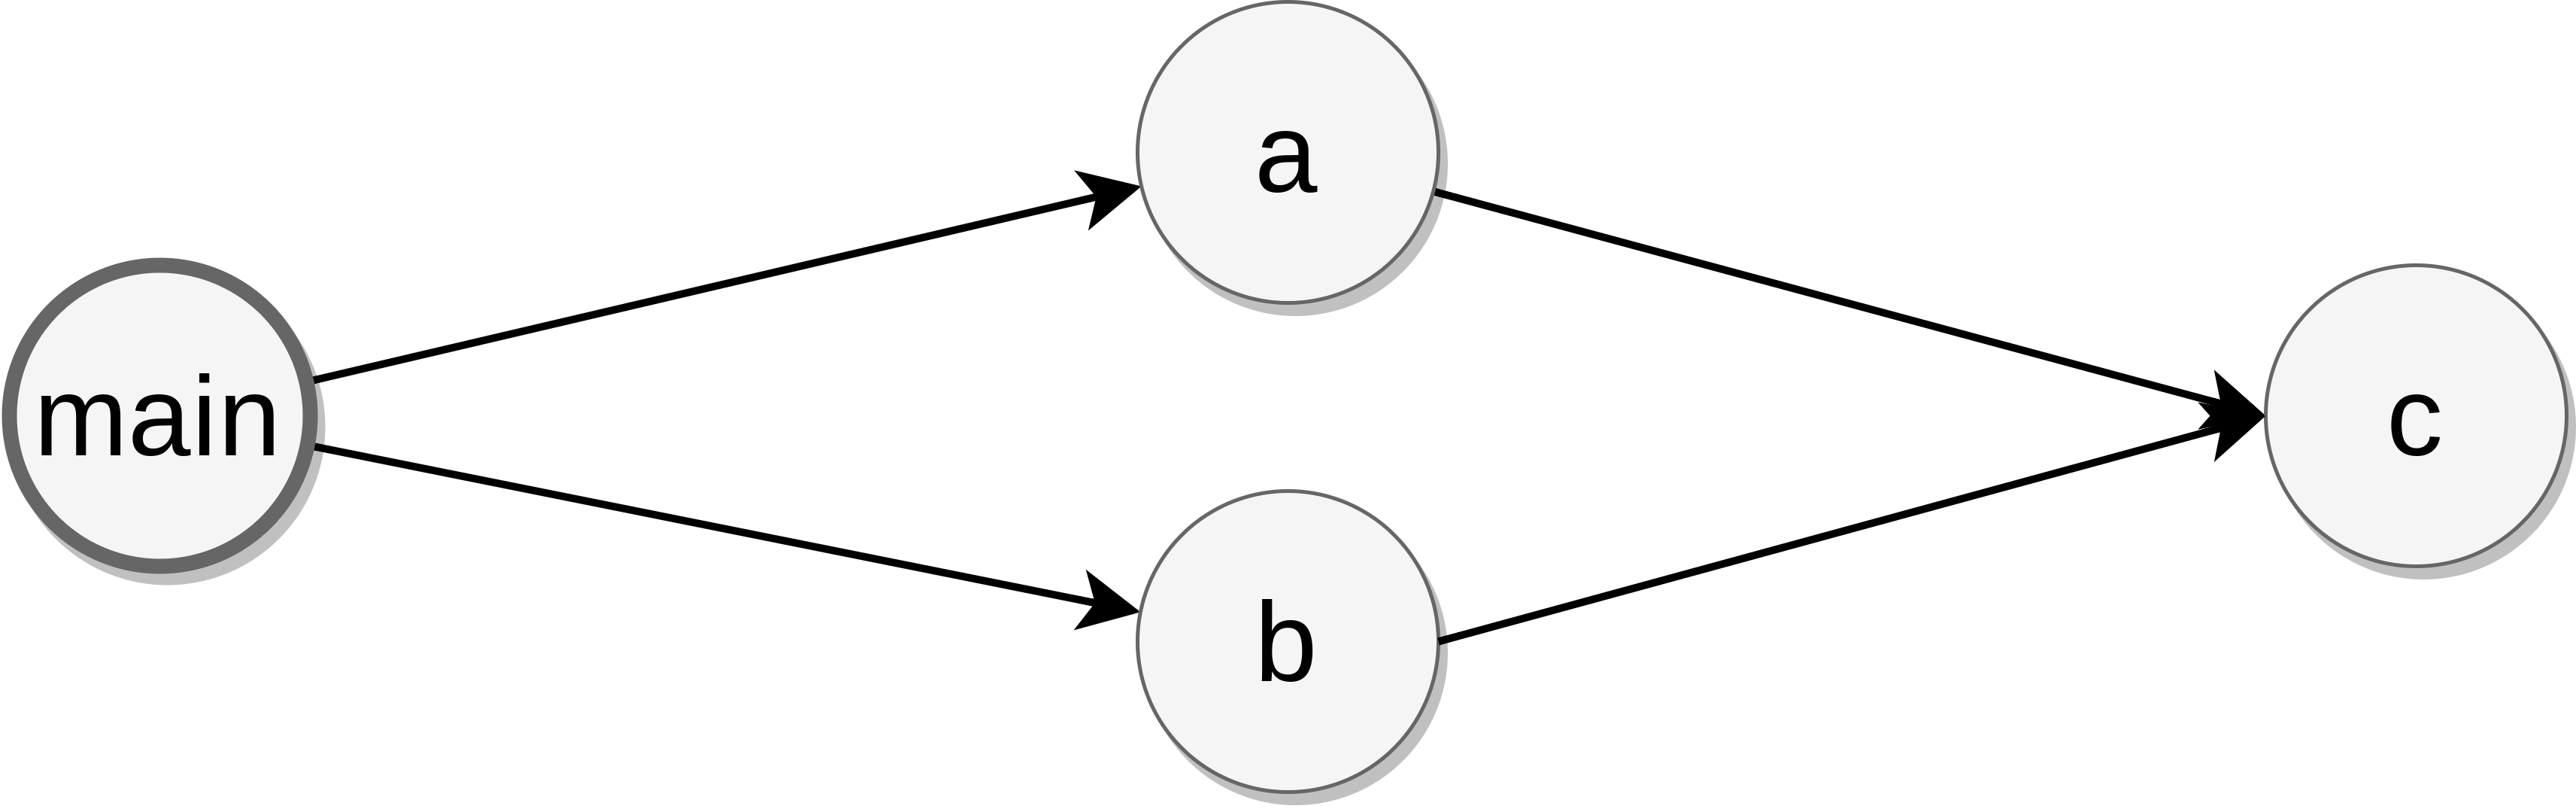
\includegraphics[width=0.8\textwidth]{../images/dependency-tree-Parallel.png}
      \end{center}
    \end{column}
  \end{columns}
\end{frame}

\begin{frame}[fragile]
  \frametitle{PDDL problem 1}

  \begin{lstlisting}[style=pddlStyle,basicstyle=\ttfamily\fontsize{10pt}{10pt}\selectfont]
    (:init
        (executed_instruction id0)

        (assignment_id assignmentA id1)
        (assignment_id assignmentB id2)
        (operation_id sumAB id3)
        (assignment_id assignmentC id4)
        
        (dependency_tree id0 id1)
        (dependency_tree id0 id2)
        (dependency_tree id1 id3)
        (dependency_tree id2 id3)
        (dependency_tree id3 id4)
    )

    (:goal (and
        (executed_assignment assignmentA)
        (executed_assignment assignmentB)
        (executed_binary_operation assignmentA assignmentB sumAB assignmentC)
        (executed_assignment assignmentC)
    ))
  \end{lstlisting}
\end{frame}

\begin{frame}[fragile]
  \frametitle{PDDL problem 1}

  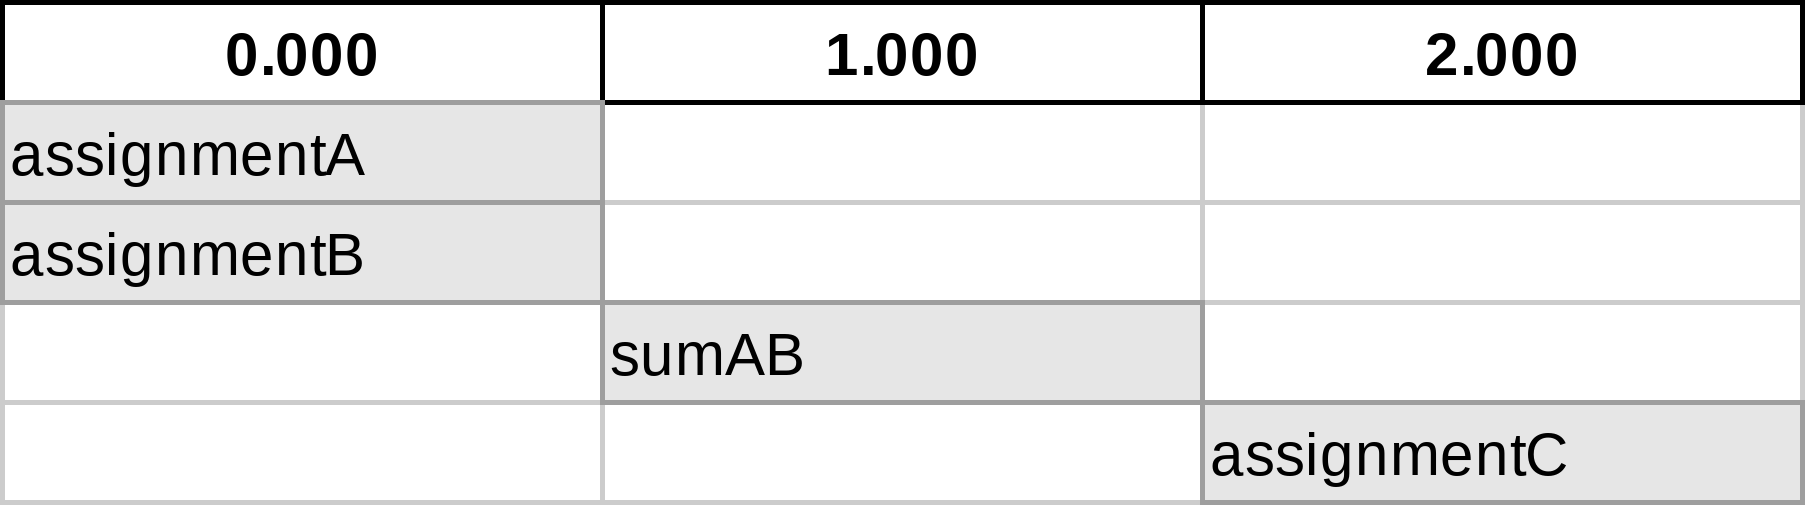
\includegraphics[width=1\textwidth]{../images/parallel-tasks-Parallel.png}
\end{frame}

\begin{frame}[fragile]
  \frametitle{PDDL problem 2}

  \begin{columns}
    \begin{column}{0.35\textwidth}
      \begin{lstlisting}[style=cppStyle]
        int main()
        {
          int a = 3;
          int b = a + 1;
          int c = a + b;
          return 0;
        }
      \end{lstlisting}
    \end{column}
    \begin{column}{0.65\textwidth}
      \begin{center}
        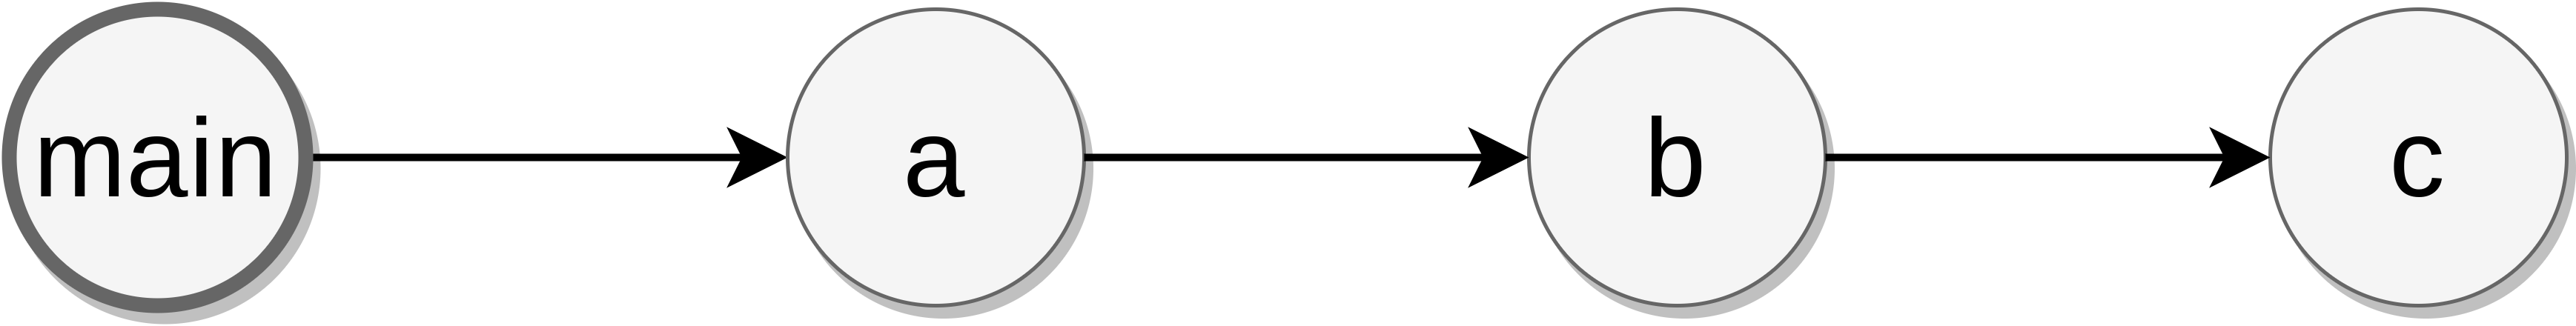
\includegraphics[width=0.8\textwidth]{../images/dependency-tree-NotParallel.png}
      \end{center}
    \end{column}
  \end{columns}
\end{frame}

\begin{frame}[fragile]
  \frametitle{PDDL problem 2}

  \begin{lstlisting}[style=pddlStyle,basicstyle=\ttfamily\fontsize{10pt}{10pt}\selectfont]
    (:init
        (executed_instruction id0)

        (assignment_id assignmentA id1)
        (assignment_id assignmentB id2)
        (operation_id sumAB id3)
        (assignment_id assignmentC id4)
        
        (dependency_tree id0 id1)
        (dependency_tree id1 id2)
        (dependency_tree id1 id3)
        (dependency_tree id2 id3)
        (dependency_tree id3 id4)
    )

    (:goal (and
        (executed_assignment assignmentA)
        (executed_assignment assignmentB)
        (executed_binary_operation assignmentA assignmentB sumAB assignmentC)
        (executed_assignment assignmentC)
    ))
  \end{lstlisting}
\end{frame}

\begin{frame}[fragile]
  \frametitle{PDDL problem 2}

  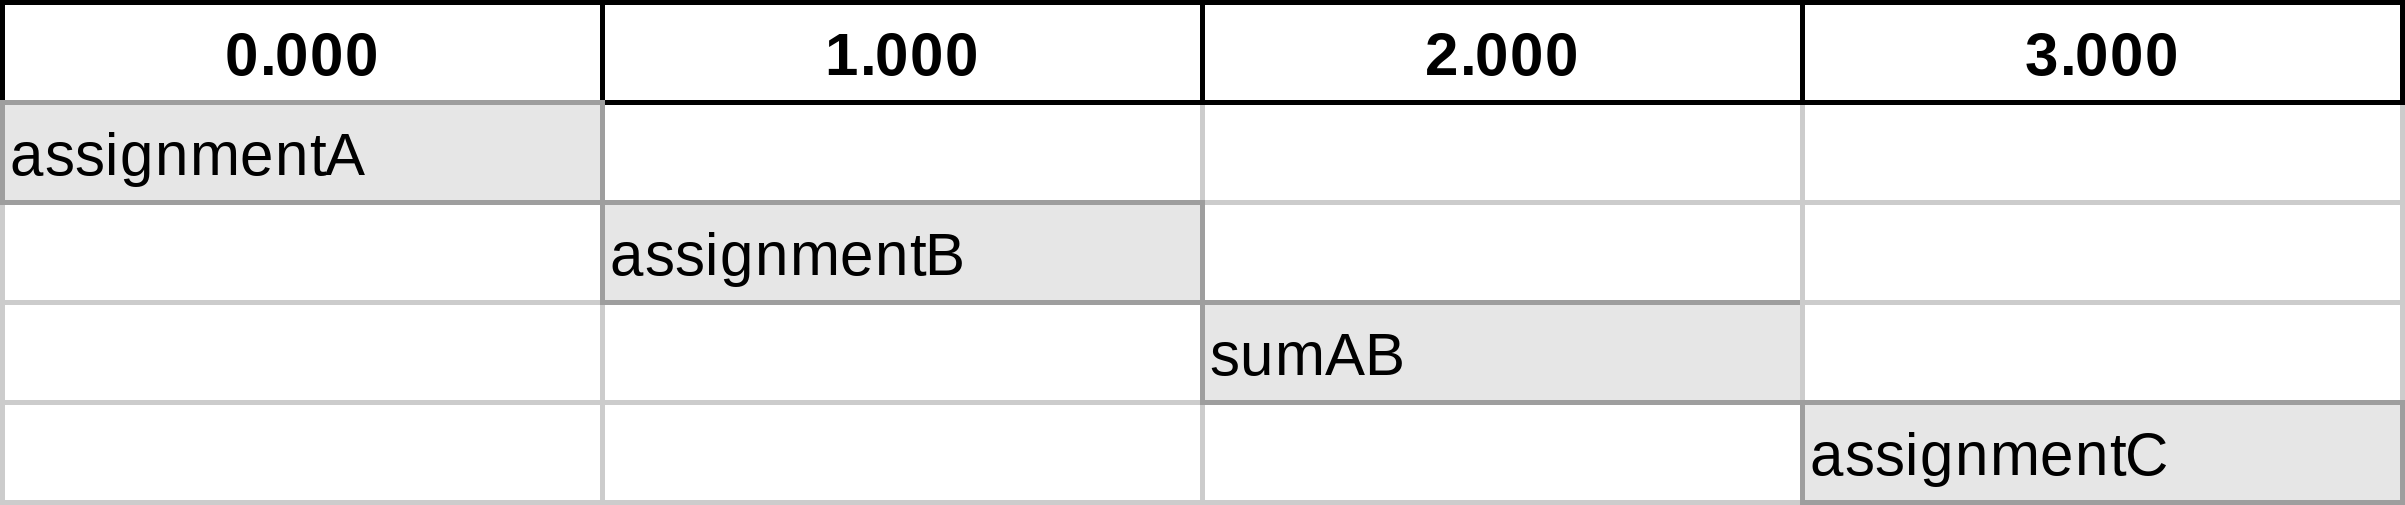
\includegraphics[width=1\textwidth]{../images/parallel-tasks-NotParallel.png}
\end{frame}
%---------------------------------------------------------


%---------------------------------------------------------
\section{Challenges}

\begin{frame}[fragile]
  \frametitle{How to handle \texttt{for} loops?}

  \begin{columns}
    \begin{column}{0.5\textwidth}
      \begin{center}
        \begin{lstlisting}[style=cppStyle,basicstyle=\ttfamily\fontsize{7.5pt}{7.5pt}\selectfont]
          int main()
          {
            int s = 0;
            std::vector<int> x = {1, 2, 3};
            for (int i = 0; i < x.size(); i++)
            {
              s += x[i];
            }
            return 0;
          }
        \end{lstlisting}
      \end{center}
    \end{column}
    \begin{column}{0.5\textwidth}
      \begin{center}
        \begin{lstlisting}[style=cppStyle,basicstyle=\ttfamily\fontsize{6.5pt}{7.5pt}\selectfont]
          int main()
          {
            int a[3] = {0};
            a[0] = rand();
            for (int i = 1; i < 3; ++i)
            {
              a[i] = a[i - 1] + rand();
            }
            return 0;
          }
        \end{lstlisting}
      \end{center}
    \end{column}
  \end{columns}
\end{frame}
%---------------------------------------------------------


%---------------------------------------------------------
\section{Questions/Ideas}

\begin{frame}
  \frametitle{Questions/Ideas}

  \begin{enumerate}
    \item<1-> Is the compiler domain capable of handling fluent variables and predicates?
    \item<2-> Is the compiler domain capable of performing operations with strings?
    \item<3-> Which planners should I test the compiler domain on?
    \item<4-> How does a planner find a parallel region?
    \item<5-> Can I set a weight for the planner to get regions that are really worth running in parallel?
  \end{enumerate}
\end{frame}
%---------------------------------------------------------


%---------------------------------------------------------
\section{Conclusion}

\begin{frame}
  \frametitle{Conclusion}

  \begin{itemize}
    \item<1-> This is not a conventional approach;
    \item<2-> If the results are positives, the approach may reduce the amount of time to find parallel regions.
  \end{itemize}
\end{frame}
%---------------------------------------------------------

\end{document}